\documentclass{article}
\usepackage{graphicx}
\usepackage{float}
\usepackage{hyperref}

\title{Assignment 1 FYS-2021}
\author{Markus Leander Wilhelmsen}
\begin{document}
\maketitle

\section{Introduction}
This assignment taught us how to extract and filter out data in python
to which can be used in a machine learning algorithm. Github link
\url{https://github.com/markuslw/FYS-2021-1}

\section{Design \& Implementation}
To retrieve data to be used in machine learning, we load a \verb|CSV| file,
filter out the relevant columns, create a new column with values to
represent the filtered columns, and create a count of the different
values. From here we create a test and train set using two new columns and
the value label.
\\
Before we push the data through the logistic regression classification
method, we define the logistic function as sigmoid's. This function's
characteristic is the S-shape curve, or the sigmoid curve. We also define
the loss function as cross entropy to minimize the probability of incorrect
predictions. We also define an accuracy function to measure the percentage
of correctly predicted instances.
\\
Finally we define the logistic discrimination classifier with
stochastic gradient descent. For each epoch we run through the
samples, getting the prediction value, updating the gradients
and the weights. Once all samples have been iterated, we use the loss
function and append the result to a list to be visualized.

\section{Performance}
\begin{figure}[H]
    \centering
    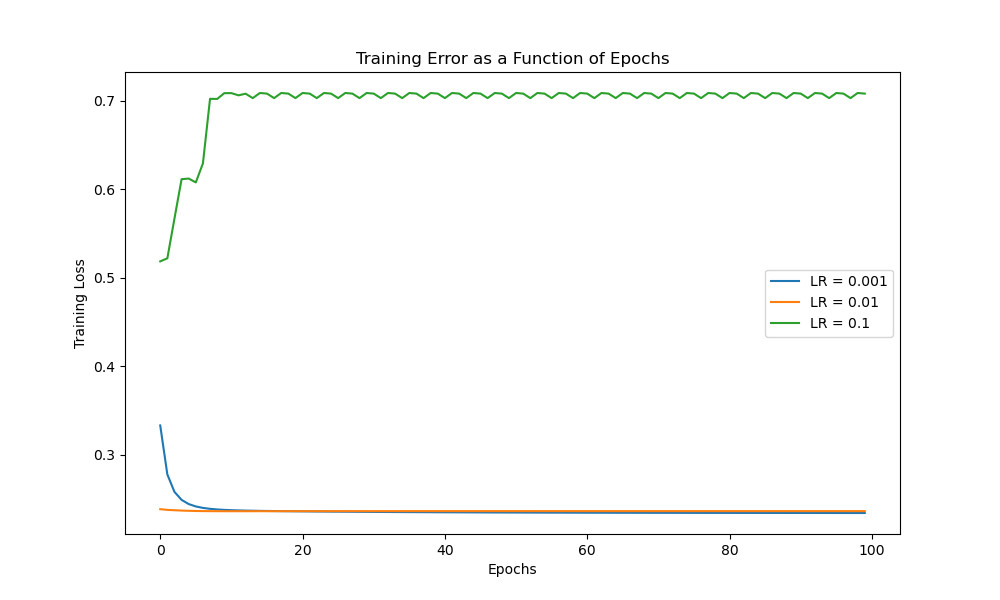
\includegraphics[width=0.8\textwidth]{../imgs/diff_lr.png} % Replace with your image name
    \caption{Learning rates visualized 0.001, 0.01, 0.1.}
\end{figure}
Figure 1 shows how with a high learning rate such as \verb|0.1|, the loss
skyrockets, fluctuates and fails to converge. The smallest rate of
\verb|0.001| shows a typical result from such a small rate, with weights
barely being updated the loss curve will appear near linear. The \verb|0.01|
rate shows that the model learns from the data and converges to minimized loss.

\bigskip

\begin{figure}[H]
    \centering
    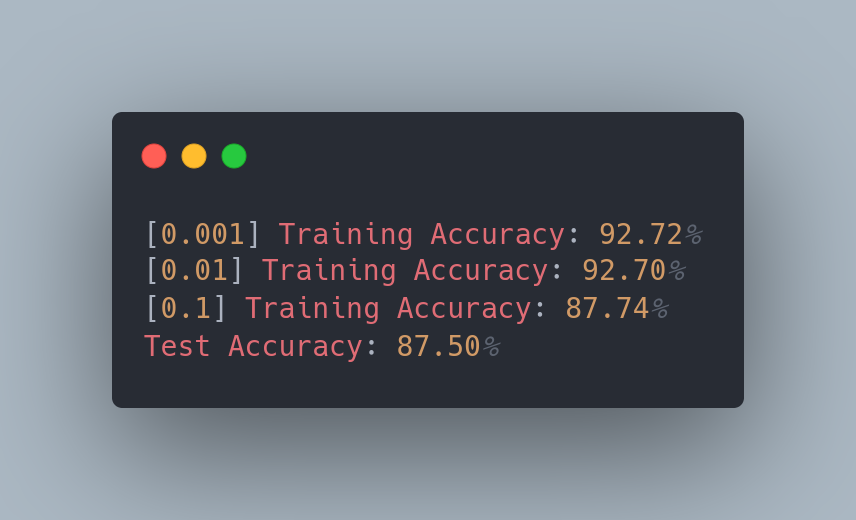
\includegraphics[width=0.8\textwidth]{../imgs/carbon1.png} % Replace with your image name
    \caption{Train and test accuracy.}
\end{figure}
Figure 2 shows the training accuracy decreasing with each step, and the
final test accuracy at 87.5\%. This reflects that with each larger step,
it tries to speed the convergence, but overshoots. The fact that the
test accuracy is lower than the training accuracy simply means it cant
generalize the data as well as on the training set.

\bigskip

\begin{figure}[H]
    \centering
    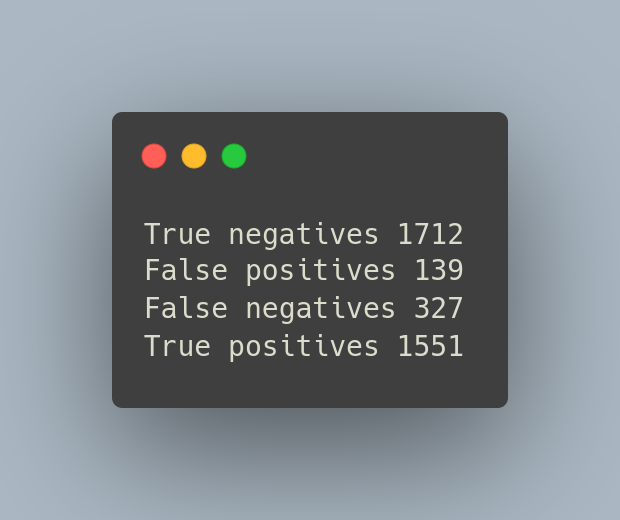
\includegraphics[width=0.8\textwidth]{../imgs/carbon2.png} % Replace with your image name
    \caption{Confusion matrix.}
\end{figure}

The confusion matrix in figure 3 provides a detailed breakdown of the accuracy
rather than just a percentage. It shows us the counts of the actual
classifications versus the predicted classifications. With the true values
being higher than its counterparts, which of course is good.

\section{References}
\begin{itemize}
    \item Lecture slide [Linear \& logistic regression]
    \item Lecture slide [Optimization and gradient descent]
    \item \url{https://www.geeksforgeeks.org/understanding-logistic-regression/}
    \item \url{https://ml-cheatsheet.readthedocs.io/en/latest/gradient_descent.html}
    \item \url{https://www2.imm.dtu.dk/pubdb/edoc/imm3274.pdf}
    \item \url{https://chandhana520.medium.com/implementing-sgd-stochastic-gradient-descent-for-linear-regression-1a82cddbb36b}
\end{itemize}
\end{document}